\section{Лабораторная работа 2 (вариант 59)}
\subsection{Задание}


Ферзь находится на поле A1 шахматной доски. Необходимо найти замкнутый маршрут из 14 ходов, обеспечивающий прохождение всех полей доски. При этом любые поля допускается проходить более одного раза.

\subsection{Результат}
\begin{verbatim}
    ?- [ferz].
    true.

    ?- run
    |    .
    Путь: [1,1,8,1,8,8,2,2,8,2,2,8,2,4,6,8,3,8,7,4,7,8,2,3,6,3,1,8,1,1]
    Путь: [1,1,8,1,8,8,3,3,7,3,2,8,2,4,6,8,3,8,7,4,7,8,1,2,7,2,1,8,1,1]
    Готово.
    true.
\end{verbatim}

Получено два варинта маршрута:

\begin{figure}[H]
\centering
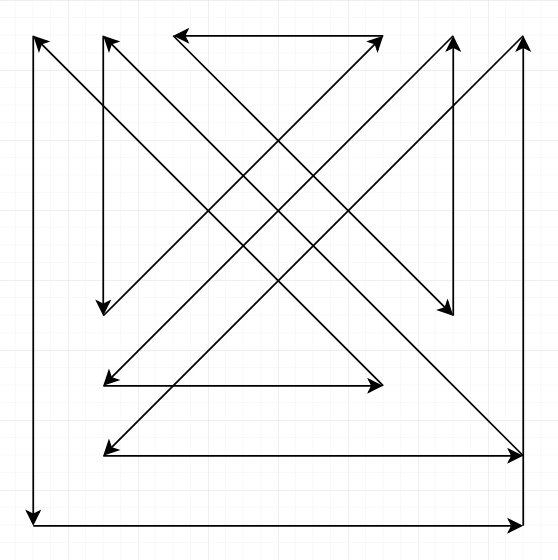
\includegraphics[scale=0.47]{way1.jpeg}
\caption{Маршрут 1}
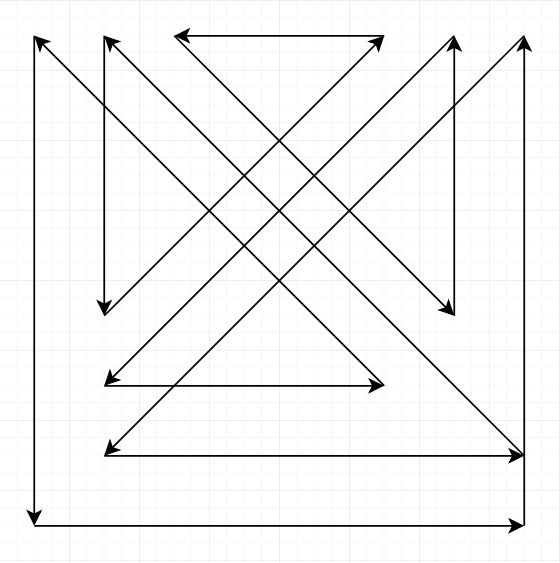
\includegraphics[scale=0.47]{way2.jpeg}
\caption{Маршрут 2}
\label{img:ways}
\end{figure}

\subsection{Иходный код}
\begin{verbatim}
     1	gen_desk(_,0,[]):-!.
     2	gen_desk(0,J,D):- J>0, J1 is J - 1, gen_desk(8, J1, D),!.
     3	gen_desk(I,J,[c(I,J,n) | D]) :- I>0, I1 is I-1, gen_desk(I1, J, D). 
     4	
     5	direction([],1):-!.
     6	direction([1],3):-!.
     7	direction([I|_],I1):- I1 is (I+3) mod 8.
     8	
     9	isEnd([]):-!.
    10	isEnd([c(_,_,y)|Desk]):-isEnd(Desk).
    11	
    12	nCoord(X,Y,X1,Y1, 0):-X<8,Y>1,X1 is X+1, Y1 is Y - 1,!.
    13	nCoord(X,Y,X1,Y,1):-X<8,X1 is X+1,!.
    14	nCoord(X,Y,X1,Y1,2):-X<8,Y<8,X1 is X+1, Y1 is Y+1,!.
    15	nCoord(X,Y,X,Y1,3):-Y<8,Y1 is Y+1,!.
    16	nCoord(X,Y,X1, Y1,4):-X>1,Y<8,X1 is X-1, Y1 is Y+1,!.
    17	nCoord(X,Y,X1, Y,5):-X>1,X1 is X-1,!.
    18	nCoord(X,Y,X1, Y1, 6):-X>1,Y>1,X1 is X-1, Y1 is Y-1,!.
    19	nCoord(X,Y,X,Y1, 7):-Y>1,Y1 is Y-1,!.
    20	
    21	broken(1,1,[],_,Desk):-isEnd(Desk).
    22	broken(X,Y,[X1,Y1|Broken],Dir,Desk):-
    23	    direction(Dir,NDir),
    24	    line(X,Y,X1,Y1,NDir,Desk,Desk1,L),
    25		L>2,
    26		broken(X1,Y1,Broken,[NDir|Dir],Desk1).
    27	
    28	line(X,Y,X0,Y0,Dir,Desk,Desk0,IJ):-
    29		nCoord(X,Y,X1,Y1,Dir),
    30	    mark(X1,Y1,Desk,Desk1,J),
    31	    line(X1,Y1,X0,Y0,Dir,Desk1,Desk0,I),
    32		IJ is I + J.
    33	line(X,Y,X,Y,_,Desk,Desk,0).
    34	
    35	mark(X,Y,[c(X,Y,n)|Desk],[c(X,Y,y)|Desk],1):-!.
    36	mark(X,Y,[c(X,Y,y)|Desk],[c(X,Y,y)|Desk],0):-!.
    37	mark(X,Y,[Cell|Desk],[Cell|Desk1],I):-mark(X,Y,Desk,Desk1,I).
    38	
    39	run :-
    40		gen_desk(8,8,Desk),
    41		broken(1,1,Broken,[],Desk),
    42		format('Путь: ~w~n', [[1,1|Broken]]),
    43		fail;
    44		write('Готово.').gen_desk(_,0,[]):-!.
    45		gen_desk(0,J,D):- J>0, J1 is J - 1, gen_desk(8, J1, D),!.
    46		gen_desk(I,J,[c(I,J,n) | D]) :- I>0, I1 is I-1, gen_desk(I1, J, D). 
\end{verbatim}

